\section{Results}
\label{sec:results}

Unless stated otherwise, results refer to the final run (\FinalTokensShort{} tokens). Table~\ref{tab:runs} summarises both runs.

\begin{table}[t]
    \centering
    \small
    % Generated by experiments/make_report_assets.py; do not edit by hand.
\begin{tabular}{lrr}
\toprule
 & Demo & Final \\
\midrule
Tokens of text8 & 1,000,000 & 5,000,000 \\
Vocabulary size & 13,966 & 36,280 \\
Tokens after subsampling & 635,140 & 3,372,979 \\
Training steps (pairs) & 11,425,544 & 60,708,682 \\
Training time & 4.2 min & 24.7 min \\
Throughput (steps/s) & 45,500 & 40,900 \\
\midrule
Mean loss, epoch 1 & 2.591 & 2.347 \\
Mean loss, epoch 2 & 2.424 & 2.250 \\
Mean loss, epoch 3 & 2.468 & 2.299 \\
\midrule
Random-pair cosine (top 2,000) & 0.61 $\pm$ 0.19 & 0.32 $\pm$ 0.12 \\
Analogies: hit@1 / hit@5 & 0 / 2 of 8 & 4 / 6 of 8 \\
\bottomrule
\end{tabular}

    \caption{Summary of the two runs. The only difference in configuration is the number of tokens.}
    \label{tab:runs}
\end{table}

\subsection{Training loss (Q1)}
\label{sec:results-loss}

\begin{figure}[t]
    \centering
    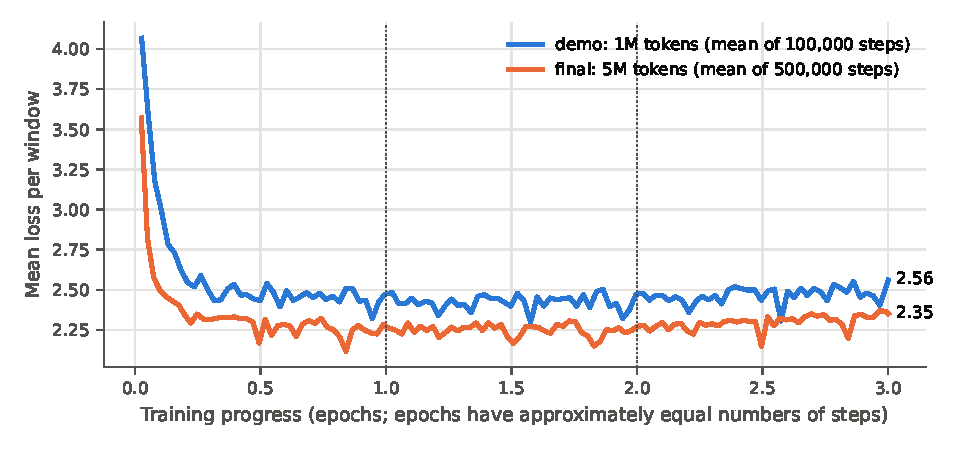
\includegraphics[width=\linewidth]{loss_curves.pdf}
    \caption{Mean training loss per window of steps. Dotted lines mark epoch boundaries; the epochs of a run have approximately equal numbers of steps.}
    \label{fig:loss}
\end{figure}

Figure~\ref{fig:loss} shows that the loss falls quickly at the start of training, from \FinalLossFirstWindow{} in the first window of the final run (\DemoLossFirstWindow{} in the demo run) to about 2.3 (about 2.45 in the demo run), and is nearly flat afterwards. Most of the decrease happens in the first quarter of the first epoch. The two curves are not directly comparable, because the final run sees text that the demo run never sees.

The epoch means in Table~\ref{tab:runs} are more surprising. Every epoch passes over the same text in the same order, so they are comparable within a run: the loss drops from epoch 1 to epoch 2 but \emph{rises} again in epoch 3, in both runs (\FinalLossEpochTwo{} to \FinalLossEpochThree{} for the final run). This is not caused by our modifications: the original code on the demo configuration gives the same pattern (2.425 to 2.469). We have not established the cause. One possible explanation is that the loss is measured on each pair just before learning from it: with a large learning rate, the model adapts to the article it is reading and predicts the next pairs of that article better, an advantage that fades as the learning rate decays towards zero. Whatever the reason, the answer to Q1 is that the objective is clearly optimised early on, but the online training loss says little about how good the embeddings are, which is why we evaluate them directly.

\subsection{Nearest neighbours (Q2)}

\begin{table}[t]
    \centering
    \small
    % Generated by experiments/make_report_assets.py; do not edit by hand.
\begin{tabular}{l>{\raggedright\arraybackslash}p{0.5\linewidth}>{\raggedright\arraybackslash}p{0.28\linewidth}}
\toprule
Query & Trained (top 8) & Untrained (top 3) \\
\midrule
\textit{king} & alexius, grandson, throne, vii, emperor, pileser, aram, honorius & marpat, verbally, brando \\
\textit{computer} & computers, computing, interface, hardware, programmer, laptop, simulation, software & subunits, svenska, mausoleum \\
\textit{city} & town, edmonton, bronx, bremerhaven, suburb, kansas, aalborg, metropolitan & expect, affinity, sharp \\
\textit{france} & italy, spain, netherlands, switzerland, germany, belgium, portugal, sweden & implying, theravada, dummett \\
\textit{january} & february, december, october, june, november, july, march, april & cajun, troopers, electrophilic \\
\textit{three} & seven, four, six, two, five, hdi, unpaved, sfg & gropius, washes, claudius \\
\textit{war} & peloponnesian, ww, wwii, outbreak, veterans, boer, crimean, falklands & ashurbanipal, route, monophyletic \\
\textit{music} & jazz, musical, dance, pop, funk, folk, hop, genres & accelerators, revolutionaries, ayckbourn \\
\bottomrule
\end{tabular}

    \caption{Nearest neighbours by cosine similarity, final run and the same model before training. All 8 query words were fixed in advance.}
    \label{tab:neighbours}
\end{table}

Table~\ref{tab:neighbours} shows that training produces meaningful neighbourhoods, while the untrained model returns unrelated words. The clearest cases are closed classes of words that can replace each other in a sentence: all eight neighbours of \textit{january} are months, those of \textit{france} are European countries, and the first five neighbours of \textit{three} are numbers. Other lists mix words of the same type with topically related words: \textit{music} has genres (\textit{jazz}, \textit{pop}, \textit{folk}), \textit{computer} has \textit{hardware}, \textit{software} and \textit{programmer}, and \textit{war} has names of wars together with \textit{outbreak} and \textit{veterans}.

Some neighbours are less intuitive. \textit{King} is closest to specific monarchs and regnal terms (\textit{alexius}, \textit{throne}, \textit{vii}, \textit{honorius}) rather than to \textit{queen}, and the neighbours of \textit{three} end with rare tokens (\textit{hdi}, \textit{unpaved}) that probably come from tables of figures in country articles. With fewer tokens, the demo run had more such noise: its neighbours of \textit{three} were mostly abbreviations, and those of \textit{computer} included \textit{animation} and \textit{game}.

\subsection{Cosine similarity (Q3)}

\begin{table}[t]
    \centering
    \small
    % Generated by experiments/make_report_assets.py; do not edit by hand.
\begin{tabular}{lrrr}
\toprule
Pair & Demo (1M) & Final (5M) & Untrained \\
\midrule
\textit{king} -- \textit{queen} & 0.91 (p98) & 0.70 (p100) & 0.10 (p82) \\
\textit{man} -- \textit{woman} & 0.89 (p97) & 0.77 (p100) & $-$0.06 (p30) \\
\textit{computer} -- \textit{software} & 0.80 (p84) & 0.75 (p100) & 0.17 (p96) \\
\textit{city} -- \textit{country} & 0.78 (p81) & 0.45 (p85) & $-$0.14 (p9) \\
\textit{france} -- \textit{germany} & 0.86 (p93) & 0.76 (p100) & 0.05 (p68) \\
\textit{january} -- \textit{february} & 0.95 (p100) & 0.91 (p100) & $-$0.03 (p39) \\
\midrule
\textit{king} -- \textit{software} & 0.14 (p1) & 0.12 (p5) & 0.00 (p49) \\
\textit{computer} -- \textit{january} & 0.42 (p17) & 0.18 (p12) & 0.04 (p67) \\
\textit{music} -- \textit{france} & 0.42 (p18) & 0.25 (p32) & 0.05 (p69) \\
\bottomrule
\end{tabular}

    \caption{Cosine similarity of fixed word pairs, with its percentile pN among random pairs of the \BaselineWords{} most frequent words of the same model. Above the line: related pairs; below: unrelated control pairs. ``Untrained'' is the final model before training.}
    \label{tab:cosine}
\end{table}

In the final run, every related pair is more similar than at least \FinalRelatedPctMin\% of random pairs, and five of the six are more similar than over 99\% of them (Table~\ref{tab:cosine}). The control pairs have percentiles between \FinalControlPctMin{} and \FinalControlPctMax. Before training, the percentiles are scattered with no relation to meaning. The answer to Q3 is therefore yes, provided similarities are compared with the right reference.

The raw values show why that reference matters. The cosine of \textit{king} and \textit{queen} \emph{decreases} from the demo to the final run (0.91 to 0.70) while its percentile increases (from 98.2 to 99.7), because the typical similarity of frequent words fell from \DemoBaselineMean{} to \FinalBaselineMean{}: with more data, vectors spread out and share less of a common direction. Raw cosine values are thus not comparable across models, and a value such as 0.70 means little on its own.

\subsection{Analogies (Q4)}

\begin{table}[t]
    \centering
    \small
    \setlength{\tabcolsep}{4.5pt}
    % Generated by experiments/make_report_assets.py; do not edit by hand.
\begin{tabular}{lllrrr}
\toprule
 & & & \multicolumn{3}{c}{Rank of expected} \\
\cmidrule(l){4-6}
Analogy & Expected & Final: top 3 & Final & Demo & Untrained \\
\midrule
\textit{man} : \textit{king} :: \textit{woman} : ? & \textit{queen} & daughter, caligula, amalric & $>$10 & $>$10 & $>$10 \\
\textit{france} : \textit{paris} :: \textit{italy} : ? & \textit{rome} & interred, venice, geneva & $>$10 & $>$10 & $>$10 \\
\textit{france} : \textit{paris} :: \textit{germany} : ? & \textit{berlin} & berlin, munich, exposition & 1 & $>$10 & $>$10 \\
\textit{man} : \textit{woman} :: \textit{boy} : ? & \textit{girl} & baby, girl, marple & 2 & $>$10 & $>$10 \\
\textit{brother} : \textit{sister} :: \textit{father} : ? & \textit{mother} & mother, grandfather, parents & 1 & $>$10 & $>$10 \\
\textit{good} : \textit{better} :: \textit{bad} : ? & \textit{worse} & fare, worse, cheaper & 2 & $>$10 & $>$10 \\
\textit{big} : \textit{bigger} :: \textit{small} : ? & \textit{smaller} & smaller, parking, forested & 1 & 3 & $>$10 \\
\textit{england} : \textit{english} :: \textit{france} : ? & \textit{french} & french, spanish, portuguese & 1 & 5 & $>$10 \\
\bottomrule
\end{tabular}

    \caption{Analogies $a : b :: c : ?$ answered by the nearest word to $\mathbf{v}_b - \mathbf{v}_a + \mathbf{v}_c$. Rank of the expected answer among the ten best candidates ($>$10: not among them).}
    \label{tab:analogies}
\end{table}

The final model ranks the expected answer first for \FinalHitOne{} of the \FinalAnswerable{} analogies and within the top five for \FinalHitFive{} (Table~\ref{tab:analogies}). The demo model reaches \DemoHitOne{} and \DemoHitFive, and the untrained model none. Capital cities (\textit{paris} $\to$ \textit{berlin}), family relations (\textit{mother}), comparatives (\textit{smaller}) and nationality adjectives (\textit{french}) work. The best-known example, \textit{king} $-$ \textit{man} $+$ \textit{woman}, does not: \textit{queen} is not among the ten best answers, which start with \textit{daughter} and two historical rulers, even though \textit{king} and \textit{queen} are highly similar. The analogy \textit{france} : \textit{paris} :: \textit{italy} : \textit{rome} also fails, while the same relation works for Germany.

An offset such as \textit{king} $-$ \textit{man} only transfers to \textit{woman} if the relation is expressed consistently across many contexts. Possible reasons for the failures are the small and topically narrow corpus, in which \textit{king} occurs mostly in historical articles about specific rulers (as its neighbours suggest), and the small number of examples of each relation. \citet{mikolov2013efficient} trained on corpora orders of magnitude larger. With 8 analogies, these counts illustrate the trend from 1M to 5M tokens but are not an accuracy estimate.

\subsection{Embedding space (Q5)}

\begin{figure}[t]
    \centering
    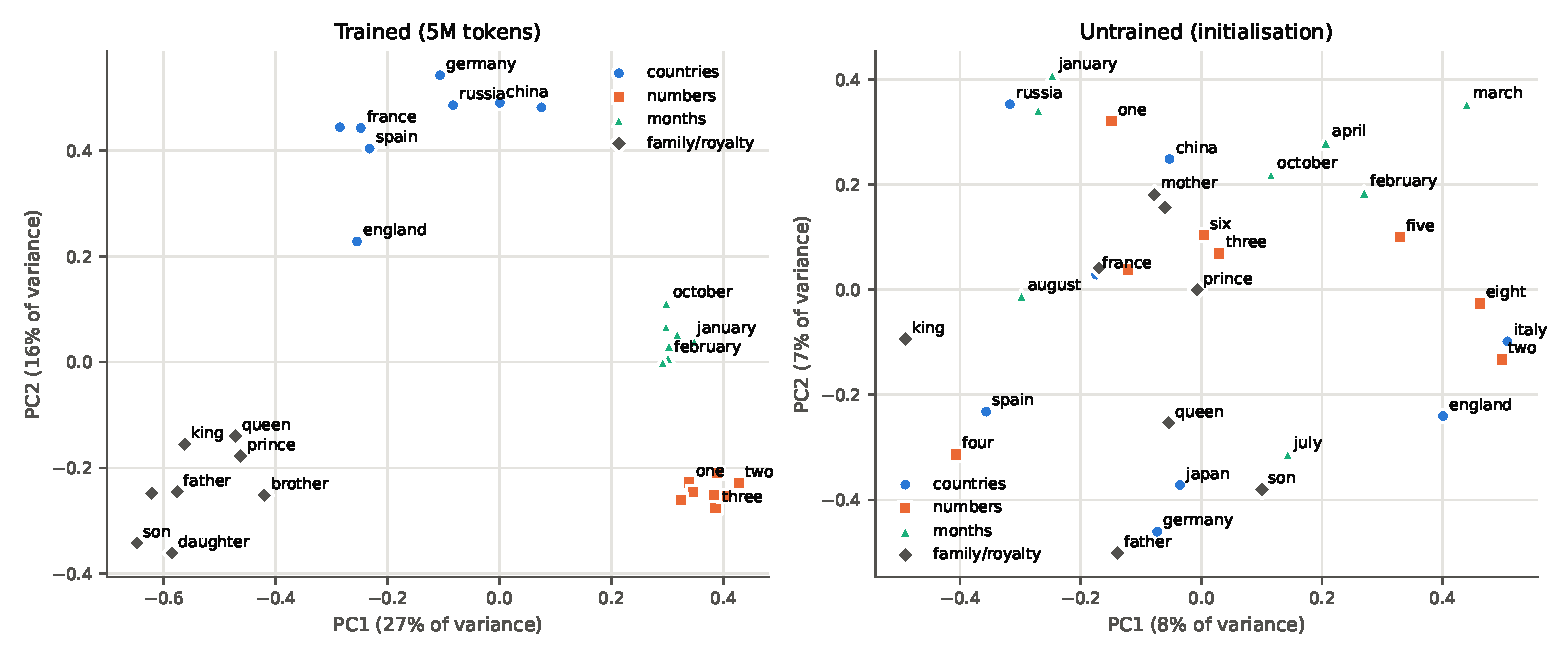
\includegraphics[width=\linewidth]{pca_final.pdf}
    \caption{PCA of 32 words from four groups fixed in advance, final model (left) and the same model before training (right). Some labels in dense clusters are omitted to avoid overlap.}
    \label{fig:pca}
\end{figure}

Figure~\ref{fig:pca} projects the 32 words of the four groups onto their first two principal components. After training, the groups form four separate clusters: numbers and months are very tight, countries are spread more widely, and family and royalty words lie together, with \textit{king}, \textit{queen} and \textit{prince} next to each other. The two components capture 27\% and 16\% of the variance of these vectors. Before training, the same words show no grouping and the components capture only 8\% and 7\%, as expected for random vectors. The picture should be read with care: the 32 words were chosen to belong to distinct groups, and two components show only part of the 100-dimensional structure.

\subsection{Effect of corpus size}

The demo and final runs share every setting except the number of tokens. Five times more text gave a vocabulary 2.6 times larger, about 5.3 times more training pairs and 5.9 times the training time (Table~\ref{tab:runs}). Every evaluation improved: neighbour lists contain less noise, related and unrelated pairs are better separated, and the analogy hits went from \DemoHitOne{}/\DemoHitFive{} to \FinalHitOne{}/\FinalHitFive{} (hit@1/hit@5). Because more text also means more updates, these two factors cannot be separated with our runs.
